\chapter{排序}

\index{排序}

\key{排序}是一个基础的算法设计问题。
许多高效的算法将排序作为子程序，
因为如果元素已经是有序的，
处理数据通常会更容易。

例如，问题''一个数组是否包含
两个相等的元素？''使用排序很容易解决。
如果数组包含两个相等的元素，
排序后它们会相邻，
因此很容易找到它们。
同样，问题''数组中出现最频繁的元素是什么？''
也可以用类似的方法解决。

排序的算法有很多种，它们也是
应用不同算法设计技术的良好示例。
高效的通用排序算法
在$O(n \log n)$时间内完成，
许多使用排序作为子程序的算法
也具有这个时间复杂度。

\section{排序理论}

排序的基本问题如下：
\begin{framed}
\noindent
给定一个包含$n$个元素的数组，
你的任务是将元素
按递增顺序排序。
\end{framed}
\noindent
例如，数组
\begin{center}
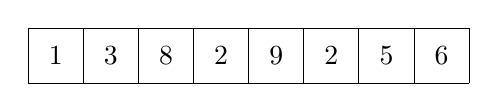
\begin{tikzpicture}[scale=0.7]
\draw (0,0) grid (8,1);
\node at (0.5,0.5) {$1$};
\node at (1.5,0.5) {$3$};
\node at (2.5,0.5) {$8$};
\node at (3.5,0.5) {$2$};
\node at (4.5,0.5) {$9$};
\node at (5.5,0.5) {$2$};
\node at (6.5,0.5) {$5$};
\node at (7.5,0.5) {$6$};
\end{tikzpicture}
\end{center}
排序后将变为：
\begin{center}
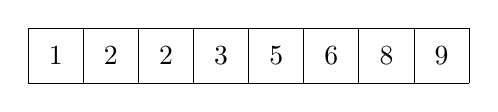
\begin{tikzpicture}[scale=0.7]
\draw (0,0) grid (8,1);
\node at (0.5,0.5) {$1$};
\node at (1.5,0.5) {$2$};
\node at (2.5,0.5) {$2$};
\node at (3.5,0.5) {$3$};
\node at (4.5,0.5) {$5$};
\node at (5.5,0.5) {$6$};
\node at (6.5,0.5) {$8$};
\node at (7.5,0.5) {$9$};
\end{tikzpicture}
\end{center}

\subsubsection{$O(n^2)$算法}

\index{冒泡排序}

简单的数组排序算法
在$O(n^2)$时间内完成。
这类算法很简短，通常
由两个嵌套循环组成。
一个著名的$O(n^2)$时间排序算法
是\key{冒泡排序}，其中元素根据其值
在数组中''冒泡''。

冒泡排序由$n$轮组成。
在每一轮中，算法遍历
数组的元素。
每当发现两个连续元素
的顺序不正确时，
算法就交换它们。
该算法可以实现如下：
\begin{lstlisting}
for (int i = 0; i < n; i++) {
    for (int j = 0; j < n-1; j++) {
        if (array[j] > array[j+1]) {
            swap(array[j],array[j+1]);
        }
    }
}
\end{lstlisting}

在算法的第一轮之后，
最大的元素将处于正确位置，
一般来说，经过$k$轮后，最大的$k$个
元素将处于正确位置。
因此，经过$n$轮后，整个数组
将被排序。

例如，在数组

\begin{center}
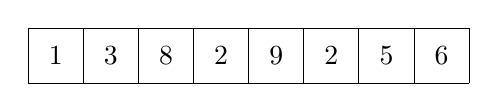
\begin{tikzpicture}[scale=0.7]
\draw (0,0) grid (8,1);

\node at (0.5,0.5) {$1$};
\node at (1.5,0.5) {$3$};
\node at (2.5,0.5) {$8$};
\node at (3.5,0.5) {$2$};
\node at (4.5,0.5) {$9$};
\node at (5.5,0.5) {$2$};
\node at (6.5,0.5) {$5$};
\node at (7.5,0.5) {$6$};
\end{tikzpicture}
\end{center}

\noindent
冒泡排序的第一轮交换元素
如下：

\begin{center}
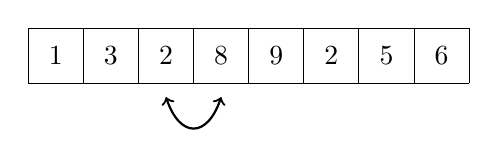
\begin{tikzpicture}[scale=0.7]
\draw (0,0) grid (8,1);
\node at (0.5,0.5) {$1$};
\node at (1.5,0.5) {$3$};
\node at (2.5,0.5) {$2$};
\node at (3.5,0.5) {$8$};
\node at (4.5,0.5) {$9$};
\node at (5.5,0.5) {$2$};
\node at (6.5,0.5) {$5$};
\node at (7.5,0.5) {$6$};

\draw[thick,<->] (3.5,-0.25) .. controls (3.25,-1.00) and (2.75,-1.00) .. (2.5,-0.25);
\end{tikzpicture}
\end{center}

\begin{center}
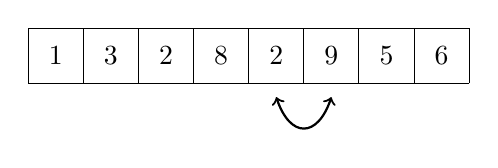
\begin{tikzpicture}[scale=0.7]
\draw (0,0) grid (8,1);
\node at (0.5,0.5) {$1$};
\node at (1.5,0.5) {$3$};
\node at (2.5,0.5) {$2$};
\node at (3.5,0.5) {$8$};
\node at (4.5,0.5) {$2$};
\node at (5.5,0.5) {$9$};
\node at (6.5,0.5) {$5$};
\node at (7.5,0.5) {$6$};

\draw[thick,<->] (5.5,-0.25) .. controls (5.25,-1.00) and (4.75,-1.00) .. (4.5,-0.25);
\end{tikzpicture}
\end{center}

\begin{center}
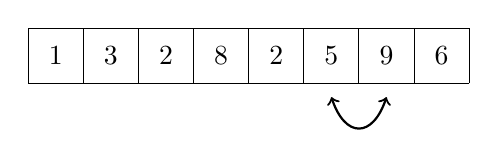
\begin{tikzpicture}[scale=0.7]
\draw (0,0) grid (8,1);
\node at (0.5,0.5) {$1$};
\node at (1.5,0.5) {$3$};
\node at (2.5,0.5) {$2$};
\node at (3.5,0.5) {$8$};
\node at (4.5,0.5) {$2$};
\node at (5.5,0.5) {$5$};
\node at (6.5,0.5) {$9$};
\node at (7.5,0.5) {$6$};

\draw[thick,<->] (6.5,-0.25) .. controls (6.25,-1.00) and (5.75,-1.00) .. (5.5,-0.25);
\end{tikzpicture}
\end{center}

\begin{center}
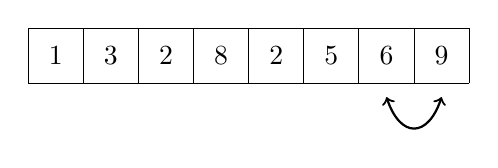
\begin{tikzpicture}[scale=0.7]
\draw (0,0) grid (8,1);
\node at (0.5,0.5) {$1$};
\node at (1.5,0.5) {$3$};
\node at (2.5,0.5) {$2$};
\node at (3.5,0.5) {$8$};
\node at (4.5,0.5) {$2$};
\node at (5.5,0.5) {$5$};
\node at (6.5,0.5) {$6$};
\node at (7.5,0.5) {$9$};

\draw[thick,<->] (7.5,-0.25) .. controls (7.25,-1.00) and (6.75,-1.00) .. (6.5,-0.25);
\end{tikzpicture}
\end{center}

\subsubsection{逆序对}

\index{逆序对}

冒泡排序是一种始终交换数组中\emph{相邻}
元素的排序算法的例子。
事实证明，这类算法的时间复杂度\emph{总是}
至少为$O(n^2)$，因为在最坏情况下，
排序数组需要$O(n^2)$次交换。

分析排序算法时的一个有用概念是\key{逆序对}：
一对数组元素
$(\texttt{array}[a],\texttt{array}[b])$，满足
$a<b$且$\texttt{array}[a]>\texttt{array}[b]$，
即元素的顺序是错误的。
例如，数组
\begin{center}
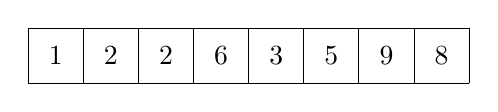
\begin{tikzpicture}[scale=0.7]
\draw (0,0) grid (8,1);
\node at (0.5,0.5) {$1$};
\node at (1.5,0.5) {$2$};
\node at (2.5,0.5) {$2$};
\node at (3.5,0.5) {$6$};
\node at (4.5,0.5) {$3$};
\node at (5.5,0.5) {$5$};
\node at (6.5,0.5) {$9$};
\node at (7.5,0.5) {$8$};
\end{tikzpicture}
\end{center}
有三个逆序对：$(6,3)$、$(6,5)$和$(9,8)$。
逆序对的数量表明
排序数组需要多少工作量。
当没有逆序对时，
数组完全有序。
另一方面，如果数组元素
是逆序排列的，
逆序对的数量达到最大：
\[1+2+\cdots+(n-1)=\frac{n(n-1)}{2} = O(n^2)\]

交换一对顺序错误的相邻元素
会从数组中恰好移除一个逆序对。
因此，如果排序算法只能交换相邻元素，
每次交换最多移除一个逆序对，
算法的时间复杂度至少为$O(n^2)$。

\subsubsection{$O(n \log n)$算法}

\index{归并排序}

使用不局限于交换相邻元素的算法，
可以在$O(n \log n)$时间内高效地对数组进行排序。
其中一个这样的算法是\key{归并排序}\footnote{根据\cite{knu983}，
归并排序由J. von Neumann于1945年发明。}，
它基于递归。

归并排序按如下方式对子数组\texttt{array}$[a \ldots b]$进行排序：

\begin{enumerate}
\item 如果$a=b$，不做任何操作，因为子数组已经有序。
\item 计算中间元素的位置：$k=\lfloor (a+b)/2 \rfloor$。
\item 递归排序子数组\texttt{array}$[a \ldots k]$。
\item 递归排序子数组\texttt{array}$[k+1 \ldots b]$。
\item 将已排序的子数组\texttt{array}$[a \ldots k]$和
\texttt{array}$[k+1 \ldots b]$
\emph{合并}为已排序的子数组\texttt{array}$[a \ldots b]$。
\end{enumerate}

归并排序是一个高效的算法，因为它
在每一步将子数组的大小减半。
递归由$O(\log n)$层组成，
处理每一层需要$O(n)$时间。
合并子数组\texttt{array}$[a \ldots k]$和\texttt{array}$[k+1 \ldots b]$
可以在线性时间内完成，因为它们已经有序。

例如，考虑对以下数组进行排序：
\begin{center}
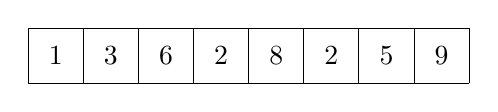
\begin{tikzpicture}[scale=0.7]
\draw (0,0) grid (8,1);
\node at (0.5,0.5) {$1$};
\node at (1.5,0.5) {$3$};
\node at (2.5,0.5) {$6$};
\node at (3.5,0.5) {$2$};
\node at (4.5,0.5) {$8$};
\node at (5.5,0.5) {$2$};
\node at (6.5,0.5) {$5$};
\node at (7.5,0.5) {$9$};
\end{tikzpicture}
\end{center}

数组将被分成两个子数组
如下：
\begin{center}
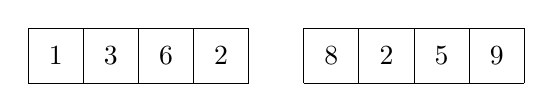
\begin{tikzpicture}[scale=0.7]
\draw (0,0) grid (4,1);
\draw (5,0) grid (9,1);

\node at (0.5,0.5) {$1$};
\node at (1.5,0.5) {$3$};
\node at (2.5,0.5) {$6$};
\node at (3.5,0.5) {$2$};

\node at (5.5,0.5) {$8$};
\node at (6.5,0.5) {$2$};
\node at (7.5,0.5) {$5$};
\node at (8.5,0.5) {$9$};
\end{tikzpicture}
\end{center}

然后，子数组将被递归排序
如下：
\begin{center}
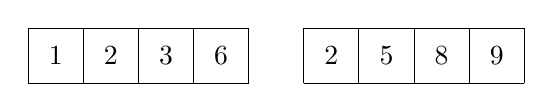
\begin{tikzpicture}[scale=0.7]
\draw (0,0) grid (4,1);
\draw (5,0) grid (9,1);

\node at (0.5,0.5) {$1$};
\node at (1.5,0.5) {$2$};
\node at (2.5,0.5) {$3$};
\node at (3.5,0.5) {$6$};

\node at (5.5,0.5) {$2$};
\node at (6.5,0.5) {$5$};
\node at (7.5,0.5) {$8$};
\node at (8.5,0.5) {$9$};
\end{tikzpicture}
\end{center}

最后，算法合并已排序的
子数组并创建最终排序的数组：
\begin{center}
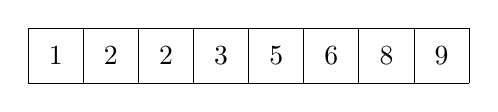
\begin{tikzpicture}[scale=0.7]
\draw (0,0) grid (8,1);
\node at (0.5,0.5) {$1$};
\node at (1.5,0.5) {$2$};
\node at (2.5,0.5) {$2$};
\node at (3.5,0.5) {$3$};
\node at (4.5,0.5) {$5$};
\node at (5.5,0.5) {$6$};
\node at (6.5,0.5) {$8$};
\node at (7.5,0.5) {$9$};
\end{tikzpicture}
\end{center}

\subsubsection{排序下界}

是否可能在快于
$O(n \log n)$的时间内对数组排序？
事实证明，当我们限定在基于比较数组元素的排序算法时，
这是\emph{不可能}的。

通过将排序视为一个过程——其中每次比较两个元素
都会给出关于数组内容的更多信息——
可以证明时间复杂度的下界。
该过程创建如下树：

\begin{center}
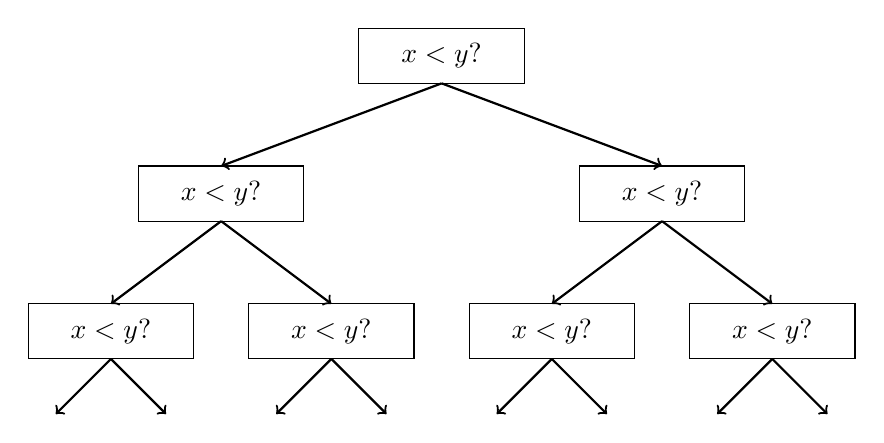
\begin{tikzpicture}[scale=0.7]
\draw (0,0) rectangle (3,1);
\node at (1.5,0.5) {$x < y?$};

\draw[thick,->] (1.5,0) -- (-2.5,-1.5);
\draw[thick,->] (1.5,0) -- (5.5,-1.5);

\draw (-4,-2.5) rectangle (-1,-1.5);
\draw (4,-2.5) rectangle (7,-1.5);
\node at (-2.5,-2) {$x < y?$};
\node at (5.5,-2) {$x < y?$};

\draw[thick,->] (-2.5,-2.5) -- (-4.5,-4);
\draw[thick,->] (-2.5,-2.5) -- (-0.5,-4);
\draw[thick,->] (5.5,-2.5) -- (3.5,-4);
\draw[thick,->] (5.5,-2.5) -- (7.5,-4);

\draw (-6,-5) rectangle (-3,-4);
\draw (-2,-5) rectangle (1,-4);
\draw (2,-5) rectangle (5,-4);
\draw (6,-5) rectangle (9,-4);
\node at (-4.5,-4.5) {$x < y?$};
\node at (-0.5,-4.5) {$x < y?$};
\node at (3.5,-4.5) {$x < y?$};
\node at (7.5,-4.5) {$x < y?$};

\draw[thick,->] (-4.5,-5) -- (-5.5,-6);
\draw[thick,->] (-4.5,-5) -- (-3.5,-6);
\draw[thick,->] (-0.5,-5) -- (0.5,-6);
\draw[thick,->] (-0.5,-5) -- (-1.5,-6);
\draw[thick,->] (3.5,-5) -- (2.5,-6);
\draw[thick,->] (3.5,-5) -- (4.5,-6);
\draw[thick,->] (7.5,-5) -- (6.5,-6);
\draw[thick,->] (7.5,-5) -- (8.5,-6);
\end{tikzpicture}
\end{center}

这里''$x<y?$''表示比较某些元素
$x$和$y$。
如果$x<y$，过程继续向左，
否则向右。
过程的结果是排序数组的可能方式，
总共有$n!$种。
因此，树的高度必须至少为
\[ \log_2(n!) = \log_2(1)+\log_2(2)+\cdots+\log_2(n).\]
我们通过选择最后的$n/2$个元素
并将每个元素的值改为$\log_2(n/2)$
来得到这个和的下界。
这给出了一个估计
\[ \log_2(n!) \ge (n/2) \cdot \log_2(n/2),\]
所以树的高度以及排序算法在最坏情况下
可能的最少步数
至少为$n \log n$。

\subsubsection{计数排序}

\index{计数排序}

下界$n \log n$不适用于
不比较数组元素而是使用其他信息的算法。
这种算法的一个例子是
\key{计数排序}，它在$O(n)$时间内对数组排序，
前提是数组中的每个元素
都是$0 \ldots c$之间的整数且$c=O(n)$。

该算法创建一个\emph{簿记}数组，
其索引是原始数组的元素。
算法遍历原始数组
并计算每个元素在数组中
出现的次数。
\newpage

例如，数组
\begin{center}
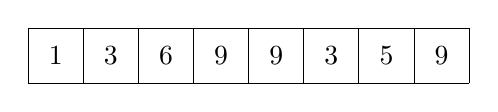
\begin{tikzpicture}[scale=0.7]
\draw (0,0) grid (8,1);
\node at (0.5,0.5) {$1$};
\node at (1.5,0.5) {$3$};
\node at (2.5,0.5) {$6$};
\node at (3.5,0.5) {$9$};
\node at (4.5,0.5) {$9$};
\node at (5.5,0.5) {$3$};
\node at (6.5,0.5) {$5$};
\node at (7.5,0.5) {$9$};
\end{tikzpicture}
\end{center}
对应以下簿记数组：
\begin{center}
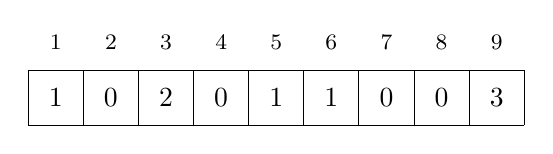
\begin{tikzpicture}[scale=0.7]
\draw (0,0) grid (9,1);
\node at (0.5,0.5) {$1$};
\node at (1.5,0.5) {$0$};
\node at (2.5,0.5) {$2$};
\node at (3.5,0.5) {$0$};
\node at (4.5,0.5) {$1$};
\node at (5.5,0.5) {$1$};
\node at (6.5,0.5) {$0$};
\node at (7.5,0.5) {$0$};
\node at (8.5,0.5) {$3$};

\footnotesize

\node at (0.5,1.5) {$1$};
\node at (1.5,1.5) {$2$};
\node at (2.5,1.5) {$3$};
\node at (3.5,1.5) {$4$};
\node at (4.5,1.5) {$5$};
\node at (5.5,1.5) {$6$};
\node at (6.5,1.5) {$7$};
\node at (7.5,1.5) {$8$};
\node at (8.5,1.5) {$9$};
\end{tikzpicture}
\end{center}

例如，簿记数组中位置3的值
为2，因为元素3在原始数组中
出现了2次。

构造簿记数组需要$O(n)$时间。
之后，可以在$O(n)$时间内创建排序后的数组，
因为可以从簿记数组中
获取每个元素的出现次数。
因此，计数排序的总时间复杂度为$O(n)$。

计数排序是一个非常高效的算法，
但它只能在常数$c$足够小的时候使用，
以便数组元素可以用作簿记数组的索引。

\section{C++中的排序}

\index{sort@\texttt{sort}}

在竞赛中几乎从不是一个好主意
去使用自制排序算法，
因为编程语言中已经有了
很好的实现。
例如，C++标准库包含
函数\texttt{sort}，可以轻松用于
对数组和其他数据结构进行排序。

使用库函数有很多好处。
首先，它节省时间，因为不需要
实现该函数。
其次，库的实现肯定是正确且高效的：
自制的排序函数不太可能更好。

在本节中，我们将看到如何使用
C++ \texttt{sort}函数。
以下代码按递增顺序对
向量进行排序：
\begin{lstlisting}
vector<int> v = {4,2,5,3,5,8,3};
sort(v.begin(),v.end());
\end{lstlisting}
排序后，向量的内容将变为
$[2,3,3,4,5,5,8]$。
默认排序顺序是递增的，
但可以按如下方式使用逆序：
\begin{lstlisting}
sort(v.rbegin(),v.rend());
\end{lstlisting}
普通数组可以按如下方式排序：
\begin{lstlisting}
int n = 7; // 数组大小
int a[] = {4,2,5,3,5,8,3};
sort(a,a+n);
\end{lstlisting}
\newpage
以下代码对字符串\texttt{s}进行排序：
\begin{lstlisting}
string s = "monkey";
sort(s.begin(), s.end());
\end{lstlisting}
对字符串进行排序意味着
对字符串的字符进行排序。
例如，字符串''monkey''变为''ekmnoy''。

\subsubsection{比较运算符}

\index{比较运算符}

函数\texttt{sort}要求为待排序元素的数据类型
定义\key{比较运算符}。
排序时，每当需要确定两个元素的顺序时，
就会使用该运算符。

大多数C++数据类型都有内置的比较运算符，
这些类型的元素可以自动排序。
例如，数字按值排序，
字符串按字母顺序排序。

\index{pair@\texttt{pair}}

对（\texttt{pair}）首先根据其
第一个元素（\texttt{first}）排序。
但是，如果两个对的第一个元素相等，
则根据第二个元素（\texttt{second}）排序：
\begin{lstlisting}
vector<pair<int,int>> v;
v.push_back({1,5});
v.push_back({2,3});
v.push_back({1,2});
sort(v.begin(), v.end());
\end{lstlisting}
之后，对的顺序为
$(1,2)$、$(1,5)$和$(2,3)$。

\index{tuple@\texttt{tuple}}

以类似的方式，元组（\texttt{tuple}）
首先按第一个元素排序，
其次按第二个元素排序，以此类推。\footnote{注意，在一些较旧的编译器中，
必须使用函数\texttt{make\_tuple}来创建元组，
而不是使用花括号（例如，\texttt{make\_tuple(2,1,4)}而不是\texttt{\{2,1,4\}}）。}：
\begin{lstlisting}
vector<tuple<int,int,int>> v;
v.push_back({2,1,4});
v.push_back({1,5,3});
v.push_back({2,1,3});
sort(v.begin(), v.end());
\end{lstlisting}
之后，元组的顺序为
$(1,5,3)$、$(2,1,3)$和$(2,1,4)$。

\subsubsection{用户自定义结构体}

用户自定义结构体不会自动拥有
比较运算符。
该运算符应该在结构体内部
定义为函数\texttt{operator<}，
其参数是同一类型的另一个元素。
如果元素小于参数，
运算符应返回\texttt{true}，
否则返回\texttt{false}。

例如，以下结构体\texttt{P}
包含一个点的x和y坐标。
比较运算符定义为
首先按x坐标排序，
其次按y坐标排序。

\begin{lstlisting}
struct P {
    int x, y;
    bool operator<(const P &p) {
        if (x != p.x) return x < p.x;
        else return y < p.y;
    }
};
\end{lstlisting}

\subsubsection{比较函数}

\index{比较函数}

还可以将外部
\key{比较函数}作为回调函数
传递给\texttt{sort}函数。
例如，以下比较函数\texttt{comp}
首先按字符串长度排序，
其次按字母顺序排序：

\begin{lstlisting}
bool comp(string a, string b) {
    if (a.size() != b.size()) return a.size() < b.size();
    return a < b;
}
\end{lstlisting}
现在可以按如下方式对字符串向量进行排序：
\begin{lstlisting}
sort(v.begin(), v.end(), comp);
\end{lstlisting}

\section{二分查找}

\index{二分查找}

在数组中搜索元素的通用方法是
使用\texttt{for}循环
遍历数组的元素。
例如，以下代码在数组中
搜索元素$x$：

\begin{lstlisting}
for (int i = 0; i < n; i++) {
    if (array[i] == x) {
        // 在索引i处找到x
    }
}
\end{lstlisting}

这种方法的时间复杂度为$O(n)$，
因为在最坏情况下，需要检查
数组的所有元素。
如果元素的顺序是任意的，
这也是最好的方法，因为没有额外的信息
表明应该在数组的哪里搜索元素$x$。

但是，如果数组是\emph{有序的}，
情况就不同了。
在这种情况下，可以更快地执行
搜索，因为数组中元素的顺序
会指引搜索。
以下\key{二分查找}算法
可以在$O(\log n)$时间内高效地
在有序数组中搜索元素。

\subsubsection{方法1}

二分查找的通常实现方式
类似于在字典中查找一个单词。
搜索在数组中维护一个活动区间，
初始时包含数组的所有元素。
然后，执行若干步骤，
每一步将区间的大小减半。

在每一步中，搜索检查活动区间
的中间元素。
如果中间元素就是目标元素，
搜索终止。
否则，搜索根据中间元素的值
递归地继续到区间的左半部分
或右半部分。

上述思路可以实现如下：
\begin{lstlisting}
int a = 0, b = n-1;
while (a <= b) {
    int k = (a+b)/2;
    if (array[k] == x) {
        // 在索引k处找到x
    }
    if (array[k] > x) b = k-1;
    else a = k+1;
}
\end{lstlisting}

在这个实现中，活动区间是$a \ldots b$，
初始区间为$0 \ldots n-1$。
算法在每一步将区间大小减半，
因此时间复杂度为$O(\log n)$。

\subsubsection{方法2}

另一种实现二分查找的方法
基于一种高效遍历数组元素的方式。
思路是进行跳跃，并在
接近目标元素时减慢速度。

搜索从左到右遍历数组，
初始跳跃长度为$n/2$。
在每一步中，跳跃长度将减半：
首先是$n/4$，然后是$n/8$、$n/16$等，
直到最后长度为1。
跳跃结束后，要么找到了目标元素，
要么我们知道它不在数组中。

以下代码实现了上述思想：
\begin{lstlisting}
int k = 0;
for (int b = n/2; b >= 1; b /= 2) {
    while (k+b < n && array[k+b] <= x) k += b;
}
if (array[k] == x) {
    // 在索引k处找到x
}
\end{lstlisting}

在搜索过程中，变量$b$
包含当前跳跃长度。
算法的时间复杂度为$O(\log n)$，
因为\texttt{while}循环中的代码
对每个跳跃长度最多执行两次。

\subsubsection{C++函数}

C++标准库包含以下基于二分查找的函数，
它们在对数时间内工作：

\begin{itemize}
\item \texttt{lower\_bound}返回指向
值不小于$x$的第一个数组元素的指针。
\item \texttt{upper\_bound}返回指向
值大于$x$的第一个数组元素的指针。
\item \texttt{equal\_range}返回上述两个指针。
\end{itemize}

这些函数假设数组是有序的。
如果不存在这样的元素，指针指向
数组最后一个元素之后的位置。
例如，以下代码判断
数组是否包含值为$x$的元素：

\begin{lstlisting}
auto k = lower_bound(array,array+n,x)-array;
if (k < n && array[k] == x) {
    // 在索引 k 处找到 x
}
\end{lstlisting}

然后，以下代码统计值为 $x$ 的元素个数：

\begin{lstlisting}
auto a = lower_bound(array, array+n, x);
auto b = upper_bound(array, array+n, x);
cout << b-a << "\n";
\end{lstlisting}

使用\texttt{equal\_range}，代码变得更简洁：

\begin{lstlisting}
auto r = equal_range(array, array+n, x);
cout << r.second-r.first << "\n";
\end{lstlisting}

\subsubsection{寻找最小解}

二分查找的一个重要用途是
找到\emph{函数}值发生变化的位置。
假设我们希望找到某个问题的
最小值$k$，使得它是有效解。
给定一个函数$\texttt{ok}(x)$，
如果$x$是有效解则返回\texttt{true}，
否则返回\texttt{false}。
此外，我们知道当$x<k$时$\texttt{ok}(x)$为\texttt{false}，
当$x \ge k$时为\texttt{true}。
情况如下：

\begin{center}
\begin{tabular}{r|rrrrrrrr}
$x$ & 0 & 1 & $\cdots$ & $k-1$ & $k$ & $k+1$ & $\cdots$ \\
\hline
$\texttt{ok}(x)$ & \texttt{false} & \texttt{false}
& $\cdots$ & \texttt{false} & \texttt{true} & \texttt{true} & $\cdots$ \\
\end{tabular}
\end{center}

\noindent
现在，可以使用二分查找找到$k$的值：

\begin{lstlisting}
int x = -1;
for (int b = z; b >= 1; b /= 2) {
    while (!ok(x+b)) x += b;
}
int k = x+1;
\end{lstlisting}

搜索找到最大的$x$值，使得
$\texttt{ok}(x)$为\texttt{false}。
因此，下一个值$k=x+1$
是使$\texttt{ok}(k)$为\texttt{true}
的最小可能值。
初始跳跃长度$z$必须
足够大，例如我们事先已知
$\texttt{ok}(z)$为\texttt{true}的某个值。

算法调用函数\texttt{ok}
$O(\log z)$次，因此总时间复杂度
取决于函数\texttt{ok}。
例如，如果该函数在$O(n)$时间内工作，
则总时间复杂度为$O(n \log z)$。

\subsubsection{寻找最大值}

二分查找也可以用于找到一个
先递增后递减的函数的最大值。
我们的任务是找到位置$k$，使得

\begin{itemize}
\item
当$x<k$时$f(x)<f(x+1)$，且
\item
当$x \ge k$时$f(x)>f(x+1)$。
\end{itemize}

思路是使用二分查找
找到最大的$x$值
使得$f(x)<f(x+1)$。
这意味着$k=x+1$，
因为$f(x+1)>f(x+2)$。
以下代码实现了该搜索： 

\begin{lstlisting}
int x = -1;
for (int b = z; b >= 1; b /= 2) {
    while (f(x+b) < f(x+b+1)) x += b;
}
int k = x+1;
\end{lstlisting}

注意，与普通二分查找不同，
这里不允许函数的连续值
相等。
在这种情况下，无法知道
如何继续搜索。
